\documentclass[lineno]{biometrika}

\usepackage{amsmath}
\usepackage{graphicx}
\usepackage{newtxtext}
\usepackage[subscriptcorrection]{newtxmath}

\def\Bka{{\it Biometrika}}
\newcommand{\pr}{\mathrm{pr}}
\newcommand{\LC}{\mathcal{L}}
\newcommand{\var}{\mathrm{var}}

\begin{document}

\jname{Biometrika}
\jyear{2026}
\jvol{}
\jnum{}
\cyear{2026}
\accessdate{}
%\received{}
%\revised{}

\markboth{K. W. Park}{Noisy calibration and the location of the mean}

\title{Noisy calibration, latent coverage and the location of the mean}

\author{KUN WOO PARK}
\affil{[Department, institution, postal address, country] \email{pkw31386094@gmail.com}}

\maketitle

\begin{abstract}
Prediction intervals for a latent quantity, such as the mean of an unsampled area, are often calibrated on noisy proxies with Gaussian errors. We ask how much the calibrated radius must be widened to cover the latent quantity, uniformly over bi-log-concave latent distributions, a class that contains the log-concave ones and some multimodal ones, and find that the answer is: almost nothing. At equal levels the worst-case widening is at most $c_q$ times the noise standard deviation, with an explicit sharp constant, $c_{0.9} = 0.0191$, and a calibration slack of one part in a thousand at the ninety per cent level removes it at every noise level. As a consequence, the noisy conformal threshold at a suitable rank covers the latent target with the nominal reliability even when the noise variances are heterogeneous and unknown. The widening is governed by the location of the latent mean: at distance $d$ from the boundary of the interval it is at most the noise variance divided by $2d$, and a widening of the order of the noise standard deviation requires the mean within a bounded multiple of that standard deviation of the boundary. Known variances serve efficiency: under log-concavity a computed radius shortens the noisy threshold by about ten per cent in our simulations.
\end{abstract}

\begin{keywords}
Conformal prediction; Deconvolution; Log-concavity; Measurement error; Small area estimation.
\end{keywords}

\section{Introduction}\label{sec:intro}

Suppose that a residual $W$, the latent target minus a centre fitted on independent training data, is observed only through $V = W + e$, where $e \sim N(0, D)$ is independent of $W$ and, until \S~\ref{sec:hetero}, $D$ is known. A survey statistician who calibrates a prediction interval for the true mean of an unsampled area on the direct estimates of sampled areas is in this position \citep{fay1979}, as is a conformal analyst whose calibration responses carry measurement error \citep{einbinder2024, cohen2025}. The threshold $t$ at which the noisy scores $|V|$ have coverage $p$ is observable. We ask which radius gives the latent residual coverage $q$, uniformly over a class of latent distributions.

If $W$ is symmetric and unimodal, the theorem of \citet{anderson1955} gives $\pr(|W + e| \le t) \le \pr(|W| \le t)$, so the noisy threshold is conservative \citep{einbinder2024}. Without symmetry the available transfers make no shape assumption: a median-zero noise turns a noisy level $1 - \alpha$ into a latent level $1 - 2\alpha$ \citep{guille2024}, and LatentCP \citep{zheng2026} uses a Markov-type compatibility threshold. \citet{cohen2025} estimate the noise-free threshold by deconvolution, without a latent guarantee; conformal intervals for small areas \citep{bersson2024} cover observable responses rather than latent area means; and \citet{armstrong2022} give worst-case empirical Bayes intervals for sampled units. For a fixed smooth latent distribution, Gaussian noise moves quantiles by $O(D)$ \citep{jochmans2024}.

Our message is that, under a shape restriction weaker than unimodality, noisy calibration is safe up to a correction that we compute exactly and that is negligible in practice. For bi-log-concave laws \citep{dumbgen2017}, the worst-case widening at equal levels is at most $c_q D^{1/2}$ with a sharp constant (Theorem~\ref{thm:small}); for log-concave laws at $q = 0.9$ it never exceeds $0.22\%$ of the radius. A calibration slack of order $10^{-3}$ removes it (Corollary~\ref{cor:slack}), so the noisy threshold at a suitable rank is valid for the latent target when the noise variances are heterogeneous and unknown (Proposition~\ref{prop:unknown}). The size of the widening is organized by the location of the mean: at distance $d$ from the boundary of the interval it is at most $D/(2d)$ for every $D$, an order attained by asymmetric laws with mean zero (Theorem~\ref{thm:mean}, Proposition~\ref{prop:centred}), and an order $D^{1/2}$ requires the mean within $O(D^{1/2})$ of the boundary (Theorem~\ref{thm:transition}). These are worst-case statements; a particular law with its mean near the boundary need not require any widening. Known variances then serve efficiency (\S~\ref{sec:hetero}).

\section{The sharp radius}\label{sec:setup}

Let $\LC$ be the class of log-concave laws on the real line, including point masses, and $\mathcal B \supset \LC$ the class of laws that are point masses or have a continuous distribution function $F$ with $\log F$ and $\log(1 - F)$ concave. Both classes are closed under translation and scaling, and convolution with a log-concave law preserves them \citep{saumard2019}. After scaling $t$ to $1$, write $x = D/t^2$ and let $Z \sim N(0,1)$ be independent of $W$. Define
\begin{equation}\label{eq:R}
R_{p,q}(x) = \sup\{ Q_q(|W|) : W \in \LC,\ \pr(|W + x^{1/2}Z| \le 1) \ge p \},
\end{equation}
where $Q_q$ is the lower $q$-quantile, and $R_{p,q}(x) = -\infty$ if nothing is feasible, which happens exactly when $\pr(|x^{1/2}Z| \le 1) < p$. If calibration certifies noisy coverage at least $p$ at threshold $t$, then $t\,R_{p,q}(D/t^2)$ is the smallest radius that guarantees latent coverage $q$ for every log-concave latent law; this is sharpness within the class and for one constraint, not optimality among procedures that use the whole calibration sample. We call $R_{p,q}(x) - 1$ the radius correction; it is a correction to a length, not to a coverage probability. Let $R^{\mathcal B}_{p,q}$ be defined by \eqref{eq:R} with $\mathcal B$ in place of $\LC$, so $R^{\mathcal B}_{p,q} \ge R_{p,q}$. The bounds of \S\S~\ref{sec:mean}--\ref{sec:slack} hold for $R^{\mathcal B}_{p,q}$ and are sharp as $x \to 0$ in both classes; the exact radius $R_{p,q}$ at a fixed $x$ and its computation use log-concavity. For $0 \le b < 1$ let $R^{(b)}_{p,q}(x)$ be defined by \eqref{eq:R} with the additional constraint $|E(W)| \le b$, so that $1 - b$ bounds the distance of the mean from the boundary.

Write $g_x(w) = \pr(|w + x^{1/2}Z| \le 1)$, so that the constraint in \eqref{eq:R} reads $E\{g_x(W)\} \ge p$, and let $\mathcal F$ be the family of point masses and of laws with density proportional to $e^{\beta w}$ on a segment $[a,b]$.

\begin{proposition}\label{prop:reduction}
$R_{p,q}(x) = \sup\{Q_q(|W|) : W \in \mathcal F,\ E\{g_x(W)\} \ge p\}$. The same holds for any continuous constraint kernel that vanishes at $\pm\infty$, in particular for the average kernel of \S~\ref{sec:hetero}.
\end{proposition}

The proof, in the Supplementary Material, truncates $W$ and applies the one-dimensional, one-constraint case of the localization theorem of \citet{fradelizi2004}, whose extreme points are point masses and log-affine densities on segments. For these laws the constraint is a combination of normal distribution functions, and the supremum reduces to a two-dimensional maximization of closed-form quantities.

\section{Worst-case radius correction and the location of the mean}\label{sec:mean}

\subsection{A one-sided problem}

Near each end of the interval the problem is one-sided. For $u > 0$ let $E_u$ be exponential with rate $u$, independent of $Z$, and for the exponential tail $b - E_u$ let
\[
m_u(b) = \pr(b - E_u + Z \le 0) = \Phi(-b) + e^{-ub + u^2/2}\,\Phi(b - u),
\]
which is continuous and strictly decreasing in $b$. Let $b_u(p)$ solve $m_u(b) = p$, and write $v_q(u) = b_u(q) - u^{-1}\log(1/q)$ and $k_q(u) = u^{-1} - b_u(q)$. The law $b_u(q) - E_u$ has $q$-quantile $v_q(u)$ and mean $-k_q(u)$.

\begin{lemma}\label{lem:onesided}
Let $c_{p,q} = \sup\{F_Y^{-1}(q) : Y \in \LC,\ \pr(Y + Z \le 0) \ge p\}$ and $c_q = c_{q,q}$. Then $c_{p,q} = \sup_{u > 0}\{b_u(p) - u^{-1}\log(1/q)\}$, $c_q > 0$, and $q \mapsto c_q$ is nonincreasing. The same holds with $\mathcal B$ in place of $\LC$.
\end{lemma}

\begin{lemma}\label{lem:meanonesided}
Let $e^{-1} < q < 1$ and $\kappa \ge 0$. Then
\[
\sup\{F_Y^{-1}(q) : Y \in \mathcal B,\ E(Y) \le -\kappa,\ \pr(Y + Z \le 0) \ge q\} = L_q(\kappa) = \sup\{v_q(u) : u > 0,\ k_q(u) \ge \kappa\}.
\]
The function $L_q$ is positive and nonincreasing, $L_q(\kappa) = c_q$ for $\kappa \le \kappa^*_q$, where $\kappa^*_q$ is the largest value of $k_q$ at a maximizer of $v_q$, and $\kappa L_q(\kappa) \to \{1 - \log(1/q)\}/2$ as $\kappa \to \infty$.
\end{lemma}

Both proofs, in the Supplementary Material, replace $Y$ by the exponential tail through a supergradient of $\log F_Y$ at its $q$-quantile; the replacement lies stochastically below $Y$, so it keeps the quantile, the noisy constraint and the bound on the mean, and only concavity of $\log F_Y$ is used. Ball arithmetic gives $c_{0.8} = 0.04607$, $c_{0.9} = 0.01906$ and $c_{0.95} = 0.00841$, and in double precision $\kappa^*_q = 6.81$, $20.18$ and $50.07$.

\subsection{No restriction on the mean}

\begin{theorem}\label{thm:small}
For every $q \in (0,1)$, every $x > 0$ and every $W \in \mathcal B$ with $\pr(|W + x^{1/2}Z| \le 1) \ge q$, $Q_q(|W|) \le 1 + c_q x^{1/2}$. Moreover $R_{q,q}(x) = 1 + c_q x^{1/2} + o(x^{1/2})$ as $x \to 0$, and likewise for $R^{\mathcal B}_{q,q}$.
\end{theorem}

\begin{proof}[of the upper bound]
Let $\alpha_R = \pr(W + x^{1/2}Z > 1)$ and $\alpha_L = \pr(W + x^{1/2}Z < -1)$, so that $\alpha_L + \alpha_R \le 1 - q$. The law of $Y = (W - 1)/x^{1/2}$ has $\log F_Y$ concave and $\pr(Y + Z \le 0) = 1 - \alpha_R$. By Lemma~\ref{lem:onesided}, $F_Y^{-1}(1 - \alpha_R) \le c_{1-\alpha_R} \le c_q$, that is, $\pr(W > 1 + c_q x^{1/2}) \le \alpha_R$. The same argument applied to $-W$, which uses concavity of $\log(1 - F_W)$, gives $\pr(W < -1 - c_q x^{1/2}) \le \alpha_L$, so $\pr(|W| \le 1 + c_q x^{1/2}) \ge q$.
\end{proof}

The lower bound, proved in the Supplementary Material, takes $W = 1 + x^{1/2}\{b_u(q + \eta_x) - E_u\}$ at a near-optimal rate $u$, with $\eta_x \to 0$: its density rises to a cut-off just outside the threshold, and its mean is within $O(x^{1/2})$ of the boundary. The correction is small at every noise level: at $q = 0.9$ the numerical upper bounds of the Supplementary Material show that $R_{q,q}(x) \le 1$ for $x \ge 0.013$, where Theorem~\ref{thm:small} bounds the correction by $0.22\%$, and the largest correction found by maximization over $\mathcal F$ is $0.063\%$ (Supplementary Material).

\subsection{The mean away from the boundary}

\begin{theorem}\label{thm:mean}
Let $W \in \mathcal B$ with $|E(W)| \le B$, let $\sigma > 0$ and $t > B$, and suppose that $\pr(|W + \sigma Z| \le t) \ge q$. Then
\[
Q_q(|W|) \le B + \{(t - B)^2 + \sigma^2\}^{1/2} \le t + \frac{\sigma^2}{2(t - B)}.
\]
In particular $R^{(b)}_{p,q}(x) \le 1 + x/\{2(1 - b)\}$ for all $p \ge q$ and $x > 0$, and $Q_q(|W|) \le (t^2 + \sigma^2)^{1/2}$ if $E(W) = 0$.
\end{theorem}

The proof in the Appendix bounds the score of the smoothed law by comparison with an exponential tail and uses the heat equation for quantiles \citep{steinbrecher2008} to obtain $d\{r(s) - B\}^2/ds \ge -1$ for $r(s) = Q_q(|W + s^{1/2}Z|)$. Unlike the expansion for a fixed smooth law, the bound is uniform over the class, and it needs neither unimodality nor symmetry. The order $x$ cannot be improved, even for mean-zero laws.

\begin{proposition}\label{prop:centred}
Let $X$ have density proportional to $e^{\beta X}$ on $[-\ell, 0]$ with $\beta > 0$ and $0 < \ell \le \infty$, let $W = X - E(X)$ and let $r_0 = Q_q(|W|)$. If $\pm r_0$ lie in the interior of the support of $W$, then, after scaling $W$ so that the noisy $q$-quantile of $|W + x^{1/2}Z|$ equals $1$,
\[
Q_q(|W|) = 1 + \tfrac{1}{2}\beta r_0\tanh(\beta r_0)\,x + o(x) \quad (x \to 0).
\]
For every $q \in (0,1)$ the condition holds for small $\beta\ell$, so $R^{(0)}_{q,q}(x) - 1$ is of exact order $x$.
\end{proposition}

The best coefficient in this family is $0.347$ at $q = 0.8$, attained by $W = 1 - E_1$, and $0.0747$ at $q = 0.9$, at $\beta\ell \approx 0.94$; so the worst-case coefficient over centred laws lies in $[0.347, 0.5]$ and $[0.0747, 0.5]$. Larger coefficients come with quantiles closer to the end of the support, and the correction appears only for noise much smaller than that gap.

\subsection{The transition}

\begin{theorem}\label{thm:transition}
Let $1 - e^{-1} < q < 1$, $x > 0$ and $W \in \mathcal B$ with $\pr(|W + x^{1/2}Z| \le 1) \ge q$. Then $|E(W)| < 1$, and if $\delta = Q_q(|W|) - 1 > 0$,
\begin{equation}\label{eq:necessary}
2\{1 - |E(W)|\}\delta + \delta^2 \le x .
\end{equation}
Moreover, for every $\kappa \ge 0$,
\[
\lim_{x \to 0} x^{-1/2}\{R^{(b_x)}_{q,q}(x) - 1\} = L_q(\kappa), \qquad b_x = 1 - \kappa x^{1/2},
\]
and the same limit holds with $\LC$ replaced by $\mathcal B$ in the definition of $R^{(b)}$.
\end{theorem}

By \eqref{eq:necessary}, a correction $\delta \ge a x^{1/2}$ with $0 < a < 1$ forces $1 - |E(W)| \le (1 - a^2)x^{1/2}/(2a)$, and the limit identifies the coefficient on that scale. In the original units the mean lies $\kappa D^{1/2}$ from the threshold, and the unrestricted worst case $c_q D^{1/2}$ persists until $\kappa$ exceeds $\kappa^*_q$, about $20$ noise standard deviations at $q = 0.9$; beyond it the coefficient decays like $\{1 - \log(1/q)\}/(2\kappa)$ (Fig.~\ref{fig:transition}). The first part is proved in the Appendix and the limit in the Supplementary Material.

\begin{figure}[t]
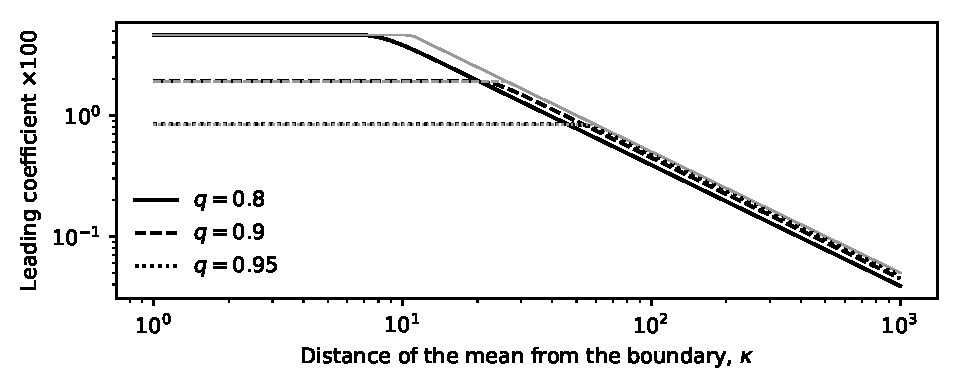
\includegraphics[width=\textwidth]{fig_transition.pdf}\global\figwidth\hsize
\caption{Leading coefficient $L_q(\kappa)$ of the worst-case radius correction, times $100$, when the mean lies at distance at least $\kappa x^{1/2}$ from the boundary (Theorem~\ref{thm:transition}), for $q = 0.8$ (solid), $0.9$ (dashes) and $0.95$ (dots), with the upper bound $\min\{c_q, (\kappa^2 + 1)^{1/2} - \kappa\}$ from Theorems~\ref{thm:small} and~\ref{thm:mean} (grey). Both axes are logarithmic.\newline Alt text: Line plot on logarithmic axes of the leading coefficient against the scaled distance of the mean from the boundary for three coverage levels. Each curve is flat at its unrestricted constant up to a threshold near 7, 20 and 50 and then decreases in proportion to the reciprocal of the distance, slightly below a grey upper bound.}
\label{fig:transition}
\end{figure}

\section{Calibration slack and a finite-sample procedure}\label{sec:procedure}

\subsection{Slack removes the correction}\label{sec:slack}

The proof of Theorem~\ref{thm:small} splits the noisy failure budget between the two ends, and it extends to $p \ge q$: for every $x$ and every $W \in \mathcal B$ feasible at level $p$,
\[
Q_q(|W|) \le 1 + C_{p,q}x^{1/2}, \qquad C_{p,q} = \sup_{\alpha_L+\alpha_R = 1-p}\ \inf_{\beta_L+\beta_R=1-q} \max(c_{1-\alpha_L,1-\beta_L},\, c_{1-\alpha_R,1-\beta_R}).
\]
Numerically the worst split puts the whole budget on one end, so that $C_{p,q} = c_{p,q}$.

\begin{corollary}\label{cor:slack}
If $C_{p,q} \le 0$ then $R^{\mathcal B}_{p,q}(x) \le 1$ for every $x$, and if $c_{p,q} > 0$ then $R_{p,q}(x) > 1$ for all small $x$. The smallest slack $p - q$ with $C_{p,q} \le 0$ lies in $(4.3\times10^{-3}, 5.0\times10^{-3}]$, $(7.9\times10^{-4}, 1.0\times10^{-3}]$ and $(1.5\times10^{-4}, 2.0\times10^{-4}]$ at $q = 0.8$, $0.9$ and $0.95$, and so does the smallest slack with $R_{q+\delta,q}(x) \le 1$ for all $x$.
\end{corollary}

Ball arithmetic also gives $-0.0572 \le C_{0.9036,0.9} \le -0.057$ and $C_{0.9068,0.9} \le -0.114$.

\subsection{Heterogeneous and unknown noise variances}\label{sec:hetero}

Let $W_1, \ldots, W_K, W_{\rm new}$ be independent with law $G$, independent of $e_i \sim N(0, D_i)$ with the $D_i$ fixed. The scores $V_i = W_i + e_i$ are independent but not identically distributed, and $\mathcal D$ denotes the calibration data.

\begin{proposition}\label{prop:beta}
Let $T = |V|_{(k)}$, let $\bar F$ be the average distribution function of the $|V_i|$, assumed continuous, and let $p_k$ be the $\delta$-quantile of the Beta$(k, K+1-k)$ distribution. If $k \ge Kp_k + 1$ then $\pr\{\bar F(T) \ge p_k\} \ge 1 - \delta$.
\end{proposition}

The proof, by \citet{hoeffding1956}, is in the Supplementary Material; the result is a case of the comparison of \citet{sen1970}.

\begin{proposition}\label{prop:unknown}
Let $G \in \mathcal B$, let the $D_i$ be unknown, and suppose that $k \ge Kp_k + 1$ and $C_{p_k,q} \le 0$. Then $\pr_{\mathcal D}\{\pr(|W_{\rm new}| \le T \mid \mathcal D) \ge q\} \ge 1 - \delta$.
\end{proposition}

\begin{proof}
On the event of Proposition~\ref{prop:beta}, $K^{-1}\sum_i \pr(|W + e_i| \le T) \ge p_k$ for $W \sim G$. If $\pr(|W| \le T) < q$, Corollary~\ref{cor:slack} at threshold $T$ gives $\pr(|W + e_i| \le T) < p_k$ for every $i$, whatever $D_i$, and so for the average, a contradiction.
\end{proof}

At $q = 0.9$ and $\delta = 0.05$ the conditions hold at the smallest rank with $p_k \ge 0.901$ and $k \ge Kp_k + 1$, which exists if and only if $K \ge 29$; for $K \le 3000$ it is at most three ranks above the usual rank with $p_k \ge 0.9$. For $K = 110$ the two coincide, at $k = 105$ with $p_k = 0.9068$. Known variances shorten the threshold.

\begin{corollary}\label{cor:simple}
Under the conditions of Proposition~\ref{prop:unknown}, if $D_i \ge D_{\min}$ for all $i$ and $C_{p',q} < 0$ for some $p' \le p_k$, then $s = \max\{0, T + C_{p',q}D_{\min}^{1/2}\}$ has the same guarantee.
\end{corollary}

\begin{proof}
On the event of Proposition~\ref{prop:beta}, some $i$ has $\pr(|W + e_i| \le T) \ge p_k \ge p'$, and the bound of \S~\ref{sec:slack} at $x = D_i/T^2$ gives $Q_q(|W|) \le T + C_{p',q}D_i^{1/2} \le T + C_{p',q}D_{\min}^{1/2}$.
\end{proof}

At $q = 0.9$ this gives $s = T - 0.114 D_{\min}^{1/2}$; it uses one negative constant, not the smallest-variance kernel, which is not a valid plug-in (Supplementary Material). The sharpest use of known variances is the average kernel $\bar g(w) = K^{-1}\sum_i \pr(|w + e_i| \le T)$: for log-concave $G$, $\int \bar g\, dG \ge p_k$ on the event of Proposition~\ref{prop:beta}, Proposition~\ref{prop:reduction} applies, and the computed radius $s = T R^{\rm mix}_{p_k - \varepsilon, q}(D_1/T^2, \ldots, D_K/T^2)$, with $\varepsilon$ bounding a discretization error, has the same guarantee.

Three levels of support should be distinguished. Proposition~\ref{prop:unknown} and Corollary~\ref{cor:simple} rest on proofs and on constants certified in ball arithmetic. The computed radius with the exact $R^{\rm mix}$ is a valid procedure, but log-concavity of $G$ is required. Our implementation returns an upper bound on $R^{\rm mix}$ from a branch and bound whose closed forms are evaluated in double precision, with boxes cleared at a margin of $10^{-9}$; this is a numerically computed upper bound, not an interval-arithmetic certificate, and the computed radii below have this status.

\section{Numerical illustration}\label{sec:numerical}

The target is $\pr_{\mathcal D}\{\pr(W_{\rm new} \in C \mid \mathcal D) \ge 0.9\} \ge 0.95$, with $K = 110$, $\var(W) = 1$ and heterogeneous noise variances $D_i = 0.577\,L_i/E(L_i)$, $L_i$ lognormal with log-scale $0.7$. Conditional coverage is exact, from closed-form latent distribution functions, with $150$ data sets per law. Besides four common log-concave laws we use a truncated exponential law, which belongs to the extremal family $\mathcal F$; an asymmetric bimodal Gaussian mixture that is bi-log-concave but not log-concave; and a scaled $t_3$ law, which is outside $\mathcal B$. All have mean zero. We compare the three rules of \S~\ref{sec:hetero}; the Fay--Herriot tolerance interval with a parametric bootstrap \citep{chatterjee2008}; and the Markov rule applied to $\bar g_T(0) - \bar g_T(W) \ge 0$, the smallest radius the single constraint allows without a shape assumption, at rank $107$, the best of $106$--$110$ for the first four laws.

\begin{table}
\tbl{Reliability, times $100$, and mean width, in parentheses; target reliability $95$}
{\begin{tabular}{lccccc}
latent law & Markov & Fay--Herriot & noisy threshold & Corollary 2 & computed \\
normal & 100 (5.92) & 96 (3.93) & 100 (4.96) & 100 (4.90) & 98 (4.45) \\
Laplace & 100 (6.29) & 93 (3.96) & 100 (5.15) & 100 (5.09) & 99 (4.66) \\
centred gamma & 100 (6.16) & 100 (3.95) & 100 (4.97) & 100 (4.90) & 100 (4.45) \\
truncated Laplace & 100 (5.89) & 85 (3.89) & 100 (4.93) & 100 (4.87) & 97 (4.42) \\
truncated exponential & %TE%
bimodal ($\mathcal B$ only) & %BM%
$t_3$ (outside $\mathcal B$) & %T3%
\end{tabular}}
\label{tab:synth}
\begin{tabnote}
Noisy threshold, $T$ at rank $105$; computed, $T R^{\rm mix}$; centred gamma with shape $2$; truncated exponential, standardized density proportional to $e^{4w}$ on $[0,1]$; bimodal, $0.4\,N(-0.95, 0.63^2) + 0.6\,N(0.63, 0.63^2)$. The computed radius has no guarantee under the bimodal and $t_3$ laws, and none of the rules has one under $t_3$. Standard errors are at most $1.8$ for reliabilities and $0.07$ for widths.
\end{tabnote}
\end{table}

%RESULTS%

\section{Discussion}\label{sec:discussion}

The guarantees are conditional on the calibration sample and concern a new area whose residual is drawn from the law of the calibration residuals, not each fixed area or a fixed finite population; unsampled areas that differ systematically from sampled ones are not covered. They assume independent Gaussian noise with a bi-log-concave, and for the computed radius log-concave, latent law. The mean condition of Theorems~\ref{thm:mean} and~\ref{thm:transition} concerns the latent residual law, which an intercept in the fitted regression does not centre.

Open questions include the leading coefficient for centred laws, between $0.0747$ and $0.5$ at $q = 0.9$, a median version of Theorem~\ref{thm:mean}, which Gaussian smoothing does not preserve, a proof that $C_{p,q} = c_{p,q}$, and whether $R^{\mathcal B}_{p,q} = R_{p,q}$ at fixed $x$.

\section*{Declaration of the use of generative AI and AI-assisted technologies}

% To be written by the author.
[To be completed by the author.]

\section*{Supplementary material}\label{SM}

The Supplementary Material includes omitted proofs, the certificates, the estimated-variance procedure, further simulations and an application. Code reproducing every number is at \texttt{https://github.com/kunhailP/noisy-calibration-latent-coverage}.

\appendix

\appendixone
\section*{Appendix 1}
\subsection*{Proofs for \S~\ref{sec:mean}}

\begin{proof}[of Theorem~\ref{thm:mean}]
Let $\mu = E(W)$. If $W$ is a point mass, $Q_q(|W|) = |\mu| \le B$. Otherwise, for $s > 0$ the law of $W + s^{1/2}Z$ is in $\mathcal B$ \citep{saumard2019}, with mean $\mu$, distribution function $F_s$ and a positive smooth density $f_s$. For $r > \mu$ let $h = f_s(r)/F_s(r)$. The tangent of $\log F_s$ at $r$ gives $F_s(y) \le \min\{F_s(r)e^{h(y - r)}, 1\}$, the distribution function of an exponential tail with mean $r - \{1 + \log F_s(r)\}/h$ that lies stochastically below $W + s^{1/2}Z$, so $\mu \ge r - \{1 + \log F_s(r)\}/h$ and $h(r - \mu) \le 1$. Laws in $\mathcal B$ satisfy $f_s' \le f_s^2/F_s$ \citep{dumbgen2017}, so $(\log f_s)'(r) \le h \le 1/(r - \mu)$; applied to $-W$ this gives $(\log f_s)'(-r) \ge -1/(r + \mu)$. Hence, for $r > B$,
\[
f_s'(r) \le \frac{f_s(r)}{r - B}, \qquad -f_s'(-r) \le \frac{f_s(-r)}{r - B}.
\]
Let $H_s(r) = \pr(|W + s^{1/2}Z| \le r)$. By the heat equation $\partial_s f_s = f_s''/2$,
\[
\partial_s H_s(r) = \tfrac12\{f_s'(r) - f_s'(-r)\} \le \frac{f_s(r) + f_s(-r)}{2(r - B)} = \frac{\partial_r H_s(r)}{2(r - B)}.
\]
The quantile $r(s) = Q_q(|W + s^{1/2}Z|)$ solves $H_s\{r(s)\} = q$ and is continuously differentiable on $s > 0$, with $r'(s) \ge -1/[2\{r(s) - B\}]$ where $r(s) > B$. Hence $\{r(s) - B\}_+^2$ has derivative at least $-1$ almost everywhere, and $\{r(\epsilon) - B\}_+^2 \le \{r(\sigma^2) - B\}_+^2 + \sigma^2 - \epsilon$. As $\epsilon \to 0$, $r(\epsilon) \to Q_q(|W|)$, because a nondegenerate law in $\mathcal B$ has a positive density on the interior of its support \citep{dumbgen2017}, so the distribution function of $|W|$ is continuous and strictly increasing where it lies strictly between $0$ and $1$. Since $r(\sigma^2) \le t$, the first inequality follows, and the second from $(d^2 + \sigma^2)^{1/2} \le d + \sigma^2/(2d)$.
\end{proof}

\begin{proof}[of Theorem~\ref{thm:transition}, first part]
Let $V = W + x^{1/2}Z$ with distribution function $F$. Since $\log F$ and $\log(1 - F)$ are concave and $F(V)$ is uniform, $E\{\log F(V)\} = -1$ and Jensen's inequality gives $F\{E(V)\} \ge e^{-1}$ and likewise $1 - F\{E(V)\} \ge e^{-1}$. If $E(W) \ge 1$ then $\pr(|V| \le 1) \le F\{E(W)\} \le 1 - e^{-1} < q$, and similarly if $E(W) \le -1$; so $|E(W)| < 1$. Theorem~\ref{thm:mean} with $B = |E(W)|$ and $t = 1$ gives $\delta \le \{d^2 + x\}^{1/2} - d$ with $d = 1 - |E(W)|$, which is \eqref{eq:necessary}.
\end{proof}

\bibliographystyle{biometrika}
\bibliography{refs}

\end{document}
